\documentclass{szzclass}
\usepackage{dependencies/szz-math}
\usepackage[czech]{babel}

\subject{KOM}
\code{BI-WSI-SI-6}
\topic{OntoUML a jeho konstrukty, transformace do objektového modelu.}

\begin{document}

\tableofcontents
\newpage

\section{OntoUML}
OntoUML je jedním z možných nástrojů konceptuálního modelování pro popisování reálného světa. Narozdíl od UML nepopisuje třídy a objekty z programátorského hlediska, místo toho definuje objekty podle jejich vlastností a stavů.

Součástí OntoUML je Unified Foundational Ontology (UFO), ta se dělá na tři části:
\begin{enumerate}
  \item \textbf{UFO-A}: strukturální aspekty reality - objekty, jejich typy, podčásti a role (v OntoUML se jedná o sortály)
  \item \textbf{UFO-B}: dynamické aspekty - události, jejich části a vazby mezi nimi (non-sortály)
  \item \textbf{UFO-C}: sociální aspekty - cíle, vztahy, stavy
\end{enumerate}

Používá modální logiku (rozšíření predikátové logiky):
\begin{itemize}
  \item[$\exists$] existenční kvantifikátor
  \item[$\forall$] univerzální kvantifikátor
  \item[$\square$] nutnost - ve všech světech platí
  \item[$\Diamond$] možnost - v některém světě platí
\end{itemize}

Postup modelování:
\begin{enumerate}
\item Vytvoření slovníku pojmů.
\item Vytváření ontologie na základě ontologických vzorů.
\item Validace konceptuálního modelu se zadavatelem.
\end{enumerate}

\section{Konstrukty}

\begin{itemize}
\item \textbf{Třída} - vychází z koncepce UML, popisuje vlastnosti sdílené mezi určitými entitami - \textbf{instance třídy}.
\item \textbf{Atribut} - reprezentuje vlastnosti sdílené instancemi třídy.
\end{itemize}

\subsection{Dědění}
Dědění - Třídy sdílející společný nadtyp mohou být sdruženy v tzv. množině nadtypu (Generalization Set). Lze upřesnit na:
\begin{itemize}
\item \textbf{Complete} - Podtřídy pokrývají všechny možné instance přímé nadtřídy.\\
  \hfill (\emph{\uv{není nadtřída, která by nebyla jednou z instancí podtříd; člověk musí být muž nebo žena, ale ne nic z toho}})
\begin{figure}[!h]
  \centering
  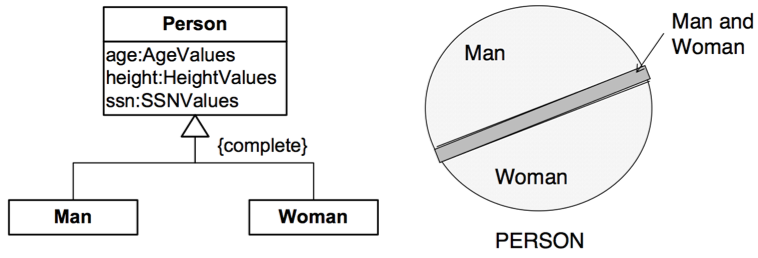
\includegraphics[width=7.5cm]{topics/bi-wsi-si-06/images/complete.png}
\end{figure}

\item \textbf{Disjoint} - všechny podmnožiny zapojené v generalizaci jsou vzájemně disjunktní\\
  \hfill (\emph{\uv{instance nemůže být obojí; člověk nemůže být muž a zároveň žena}})
\begin{figure}[!h]
  \centering
  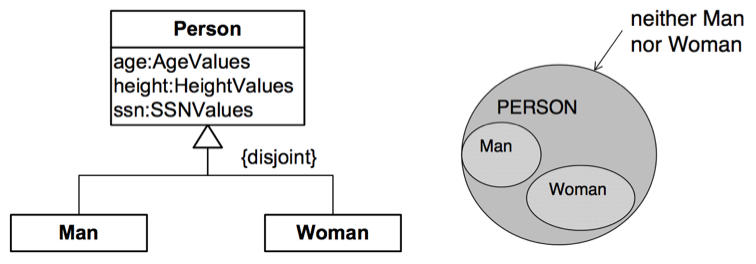
\includegraphics[width=7.5cm]{topics/bi-wsi-si-06/images/disjoint.png}
\end{figure}

\item \textbf{Complete a Disjoint} (Partition) - každá instance nadtřídy je instance právě jedné podtřídy.\\
  \hfill (\emph{\uv{Nadtřída je něco jako abstract.}})
\end{itemize}

\subsection{Typy objektů}
\begin{itemize}
\item \textbf{Sortal}
  \begin{itemize}
  \item \textbf{Rigid}
    \begin{itemize}
    \item \textbf{Kind} - poskytuje identitu
    \item \textbf{SubKind}
    \end{itemize}
  \item \textbf{Anti-rigid}
    \begin{itemize}
    \item \textbf{Phase}
    \item \textbf{Role}
    \end{itemize}
  \end{itemize}
\item \textbf{Non-sortal}
  \begin{itemize}
  \item \textbf{Rigid}
    \begin{itemize}
    \item \textbf{Category} - nutné vlastnosti více Kinds.
    \end{itemize}
  \item \textbf{Non-rigid}
    \begin{itemize}
    \item \textbf{Mixin} - vlastnosti více Kinds, které jsou nutné pro některé instance a možné pro jiné.
    \item \textbf{RoleMixin} - možné a relační vlastnosti sdílené entitami vícero typů.
    \end{itemize}
  \end{itemize}
\end{itemize}

\begin{figure}[h!]
  \centering
  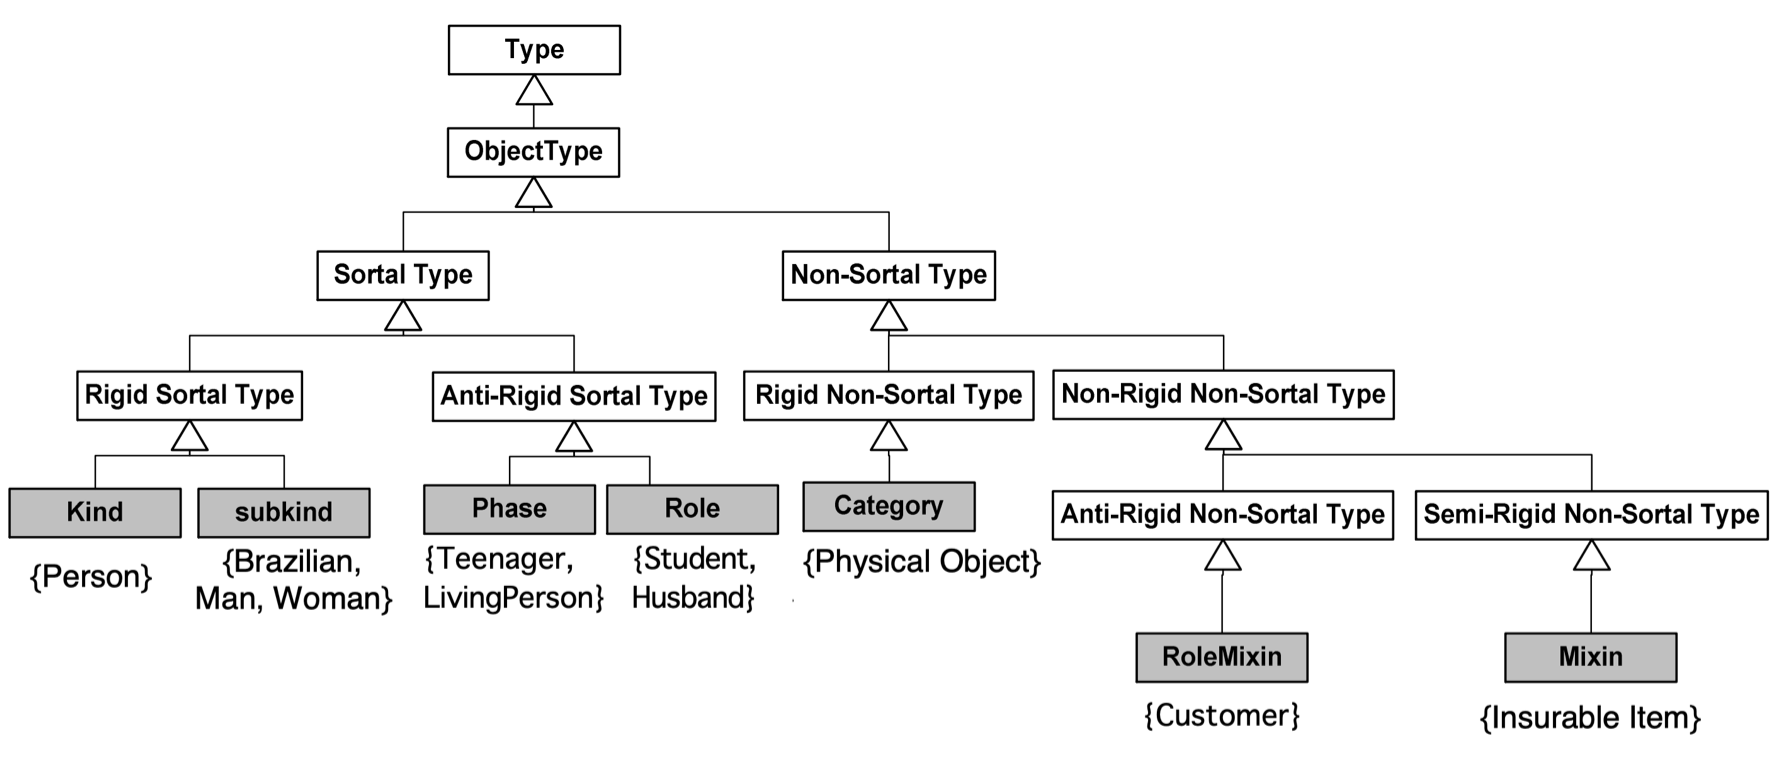
\includegraphics[width=0.8\textwidth]{topics/bi-wsi-si-06/images/type-categories}
  \caption{Kategorie typů objektů}
\end{figure}

\subsection{Sortal}
\begin{itemize}
\item \textbf{Sortal} - poskytuje identitu
\item \textbf{Non-sortal} - z hlediska našeho vnímání nemá vlastní identitu
\end{itemize}

\subsection{Rigidity}
\begin{itemize}
\item \textbf{Rigid} - Typ je rigidní pro každou instanci $x$ právě tehdy, když $x$ je nutně (v modálním slova smyslu) instancí $T$. \textit{Platí ve všech světech. Nemění se v čase.} \\
  \[
    R_+(T) \vcentcolon= \square(\forall x~T(x) \Rightarrow \square(T(x)))
  \]
\item \textbf{Anti-rigid} - Typ $T$ je anti-rigidní pro každou instanci $x$, právě tehdy když je možné (v modálním slova smyslu), že $x$ nemusí být instancí $T$. \textit{Platí v nějakém světě.} \\
  \[
    R_-(T) \vcentcolon= \square(\forall x~T(x) \Rightarrow \Diamond(\neg T(x)))
  \]
\item \textbf{Non-rigid} - logická negace rigidity.
  \[
    NR(T) \vcentcolon= \Diamond(\exists x~T(x) \Rightarrow \Diamond(\neg T(x)))
  \]
\end{itemize}

\subsection{Celek-část}
\begin{itemize}
\item \textbf{Povinná část} - Celek má alespoň jednu část
\item \textbf{Esenciální část} - Instanci části nelze měnit
\item \textbf{Nepovinný celek} - Část nepotřebuje celek
\item \textbf{Povinný celek} - Část vyžaduje celek
\item \textbf{Neoddělitelná část} - Instanci celku nelze měnit
\item \textbf{Neměnitelná část} - Část nelze měnit, celek není rigidní
\item \textbf{Neměnitelný celek} - Celek nelze měnit, část není rigidní
\end{itemize}

\begin{itemize}
\item \textbf{Quantity} - typicky materiály (např. písek, víno, dřevo, \dots); esenciální, tranzitivní, reflexivní
  \begin{itemize}
  \item \textbf{SubQuantityOf}: alkohol-víno
  \end{itemize}
\item \textbf{Collective} - 
  \begin{itemize}
  \item \textbf{MemberOf}: strom-les, student-paralelka
  \item \textbf{SubCollectionOf}: studenti s vyznamenáním-studenti
  \end{itemize}
\item \textbf{Functional Whole}
  \begin{itemize}
  \item \textbf{ComponentOf}: srdce-oběhový systém, ředitel-firma
  \end{itemize}
\end{itemize}


\section{Transformace do objektového modelu}
Transformace OntoUML do objektoveho modelu (\uv{z modelu se bude spíše odebírat}) pomocí:
\begin{itemize}
\item objektů (tříd) s atributy a metodami
\item skládání objektů
\item dědění mezi třídami
\end{itemize}

\begin{enumerate}
\item Entity $\to$ Třídy (kind, subkind, role, \dots)
\item Complete - Abstraktní třída
\item Zajištění povinnosti 1...:
  \begin{itemize}
  \item hard metoda (vynutíme v konstruktoru),
  \item soft metoda (kontrolujeme konzistenci v programu).
  \end{itemize}
\item Vztah 0...1 – instanční proměnné
\item Vztah 0...* – kolekce
\item \textbf{Complete} – nadtřída implementována jako abstraktní.
\item \textbf{Disjoint} – standardní chovaní s jednoduchou dědičností.
\item \textbf{Non-disjoint} - implementace děděním (exponenciální počet tříd) nebo skládáním.
\item \textbf{Sortal} – v implementaci jednoznačný identifikátor, který v reálném světě neexistuje.
\item \textbf{Role} – implementace jako třída, příslušnost role skládáním.
\item \textbf{Phase} – implementována návrhovým vzorem State.
\item \textbf{Non-sortal} – slouží jako další dimenze kategorizace. Zpravidla vytváří problém s vícenásobnou dědičností / skládání.
\end{enumerate}
\end{document}
